%% =======================================================
%% Actividad 9: Representación computacional de distribuciones
%%
%% Compilar desde actividades/: ./compilar.sh act09
%% Las figuras de img/ se generan con: python act09.py
%% =======================================================

%% ---- CONFIGURACIÓN ------------------------

\documentclass[11pt,letterpaper]{article}

\usepackage[indice]{tecnm}
\usepackage[T1]{fontenc}
\usepackage{amsmath}
\usepackage{xcolor}
\usepackage[most]{tcolorbox} % Carga tcolorbox con soporte para listings y saltos de página
\tcbuselibrary{listings, skins, breakable}
\setlength{\emergencystretch}{3em} % Evita líneas desbordadas por palabras en \texttt

% Paleta de colores (estilo GitHub Light / VS Code)
\definecolor{codebg}{HTML}{F8F9FA}       % Fondo del código
\definecolor{codehead}{HTML}{E9ECEF}     % Fondo de la barra de título
\definecolor{codeborder}{HTML}{CED4DA}   % Borde de la tarjeta
\definecolor{codetitle}{HTML}{212529}    % Texto del título
\definecolor{codekw}{HTML}{0550AE}       % Palabras clave (import, def, for...)
\definecolor{codefunc}{HTML}{8250DF}     % Funciones y métodos (describe, groupby...)
\definecolor{codestr}{HTML}{0A3069}      % Strings
\definecolor{codecomm}{HTML}{6E7781}     % Comentarios
\definecolor{codenum}{HTML}{8C959F}      % Números de línea
\definecolor{codeid}{HTML}{24292F}       % Texto general

% Configuración base de listings
\lstdefinestyle{pythonestilo}{
  language=Python,
  basicstyle=\ttfamily\footnotesize\color{codeid},
  keywordstyle=\color{codekw}\bfseries,
  keywordstyle=[2]\color{codefunc}, % Estilo secundario para métodos de datos
  stringstyle=\color{teal!80!black},
  commentstyle=\color{codecomm}\itshape,
  morekeywords={as, True, False, None, with, yield, lambda},
  morekeywords=[2]{print, len, sum, max, DataFrame, Series, value_counts, reindex, mean, std, var, randint, normal, seed, cumsum, poisson, binom, pmf, norm, fit, kde, bincount, linspace, train_test_split, make_blobs, GaussianNB, chisquare, pdf, cdf, hist, bar, plot, axhline, axvline, fill_between, subplots, figure, concat, nunique, load_iris, diff, sort, unique},
  numbers=left,
  numberstyle=\tiny\ttfamily\color{codenum},
  stepnumber=1,
  numbersep=10pt,
  showstringspaces=false,
  morestring=[b]{"""},
  tabsize=4,
  breaklines=true,
  breakatwhitespace=true,
  columns=flexible,
  keepspaces=true,
  literate=
    {á}{{\'a}}1 {é}{{\'e}}1 {í}{{\'i}}1 {ó}{{\'o}}1 {ú}{{\'u}}1
    {Á}{{\'A}}1 {É}{{\'E}}1 {Í}{{\'I}}1 {Ó}{{\'O}}1 {Ú}{{\'U}}1
    {ñ}{{\~n}}1 {Ñ}{{\~N}}1 {¿}{{?`}}1 {¡}{{!`}}1 {°}{{$^\circ$}}1
}

% Definición del entorno personalizado \begin{codigo}{Título}{etiqueta}
% \newtcblisting[auto counter, number within=section]{codigo}[2][]{
\newtcblisting[auto counter]{codigo}[2][]{
  listing only,
  breakable,                    % Permite que el bloque se divida si pasa de página
  enhanced,
  colback=codebg,
  colframe=codeborder,
  colbacktitle=codehead,
  coltitle=codetitle,
  fonttitle=\bfseries\small\sffamily,
  boxrule=0.6pt,
  arc=4pt,                      % Bordes redondeados
  left=20pt,                    % Espacio izquierdo para los números de línea
  right=8pt,
  top=6pt,
  bottom=6pt,
  toptitle=4pt,
  bottomtitle=4pt,
  before skip=12pt,
  after skip=12pt,
  listing options={style=pythonestilo},
  title={Código \thetcbcounter: #2},
  #1
}

% Paleta para salida de consola (estilo terminal limpia)
\definecolor{termbg}{HTML}{212529}      % Fondo oscuro tipo terminal
\definecolor{termhead}{HTML}{343A40}    % Barra superior
\definecolor{termtext}{HTML}{F8F9FA}    % Texto claro de alta legibilidad
\definecolor{termborder}{HTML}{495057}  % Borde

% Entorno \begin{consola}[label=out:iris]{Título}
\newtcblisting[auto counter]{consola}[2][]{
  listing only,
  breakable,
  colback=termbg,
  colframe=termborder,
  colbacktitle=termhead,
  coltitle=termtext,
  colupper=termtext,
  fonttitle=\bfseries\small\sffamily,
  boxrule=0.6pt,
  arc=4pt,
  left=8pt,
  right=8pt,
  top=6pt,
  bottom=6pt,
  toptitle=4pt,
  bottomtitle=4pt,
  before skip=12pt,
  after skip=12pt,
  listing options={
    basicstyle=\ttfamily\scriptsize\color{termtext}, % \scriptsize evita que las tablas de Pandas se partan de línea
    breaklines=true,
    columns=fixed,        % Mantiene alineadas las columnas de Pandas
    keepspaces=true,
    showstringspaces=false,
    literate=
      {á}{{\'a}}1 {é}{{\'e}}1 {í}{{\'i}}1 {ó}{{\'o}}1 {ú}{{\'u}}1
      {Á}{{\'A}}1 {É}{{\'E}}1 {Í}{{\'I}}1 {Ó}{{\'O}}1 {Ú}{{\'U}}1
      {ñ}{{\~n}}1 {Ñ}{{\~N}}1 {°}{{$^\circ$}}1
  },
  title={Salida \thetcbcounter: #2},
  #1
}

%% ---- DATOS DE LA MATERIA ------------------------

\materia{Modelos Estadísticos para el Aprendizaje \\ Automático y Ciencia de Datos}
\actividad{Tema 2.1
Variables Aleatorias: Tipos, Ejemplos, Representación Computacional \\ Actividad 9 - Representación Computacional de Distribuciones}

\profesor{Dr. José Ismael Ojeda Campaña}
%\fecha{15 de octubre de 2026}    % opcional; por defecto es la fecha de hoy

\begin{document}
\portada
\indicegeneral

%% ---- CONTENIDO ---------------------------------

\section{Introducción}

Cada distribución de probabilidad tiene parámetros que determinan su forma: dónde se centra, qué tan dispersa es y qué tan simétrica resulta. Entender cómo cambian esas formas al variar los parámetros es necesario para elegir la distribución adecuada para una variable aleatoria y, después, para construir modelos predictivos sobre ella \parencite{tecnm2026_documento_fuente,brownlee2020}.

En este documento se manipulan los parámetros de dos distribuciones y se visualiza su efecto. Primero se generan muestras de distribuciones normales con medias 0, 5 y 10 y desviaciones estándar 1, 2 y 3, y se superponen sus curvas de densidad. Después se simulan datos de la distribución de Poisson con $\lambda = 1, 5$ y $10$ y se comparan con distribuciones binomiales de la misma media. Finalmente, se ajusta una distribución normal a la temperatura del Weather Dataset \parencite{witten2017} y se evalúa visualmente qué tan bien describe los datos.

\section{Marco conceptual}

\subsection{Distribuciones de probabilidad discretas y continuas}

Una distribución de probabilidad es un resumen de las probabilidades para los valores de una variable aleatoria. Si la variable es discreta, la distribución se resume con una función de masa de probabilidad; entre las más conocidas están la de Poisson, la de Bernoulli y la binomial. Si es continua, se resume con una función de densidad; algunos ejemplos son la normal o gaussiana, la exponencial y la gamma \parencite{tecnm2026_documento_fuente,brownlee2020}.

\subsection{Distribución normal}

La distribución normal está determinada por dos parámetros, la media $\mu$ y la desviación estándar $\sigma$, y su densidad es
\begin{equation}
    f(x) = \frac{1}{\sigma \sqrt{2\pi}} \exp\!\left( -\frac{(x - \mu)^2}{2\sigma^2} \right).
\end{equation}
Cada parámetro tiene un efecto distinto en la forma de la curva. La media $\mu$ es el centro de simetría: cambiarla desplaza la curva sin modificar su forma. La desviación estándar $\sigma$ controla la dispersión: al aumentarla, la curva se ensancha y, como el área total debe seguir siendo 1, su altura máxima baja, $f(\mu) = 1/(\sigma\sqrt{2\pi})$ \parencite{bonamente2017}. Aproximadamente el 95\,\% de los valores queda en el intervalo $\mu \pm 1.96\,\sigma$ \parencite{bonamente2017}.

\subsection{Distribución de Poisson}

La distribución de Poisson describe el número de veces que ocurre un evento en un intervalo fijo de tiempo o espacio, cuando los eventos suceden de manera independiente y a una tasa promedio constante. Es útil para eventos raros o poco frecuentes, como las llamadas a una central telefónica o los accidentes en una carretera durante un día \parencite{tecnm2026_documento_fuente}. Su parámetro $\lambda$ es la tasa promedio de eventos en el intervalo, y la probabilidad de observar exactamente $k$ eventos es
\begin{equation}
    P(X = k) = \frac{e^{-\lambda}\,\lambda^k}{k!}, \qquad k = 0, 1, 2, \ldots
\end{equation}
Su media y su varianza son iguales a $\lambda$ \parencite{rice2006}. Cuando $\lambda$ es pequeña, la distribución es asimétrica con una cola larga a la derecha, y al aumentar $\lambda$ se vuelve más simétrica y más dispersa.

\subsection{Relación con la distribución binomial}

La distribución binomial da la probabilidad de obtener $k$ éxitos en $n$ pruebas independientes, cada una con probabilidad de éxito $p$:
\begin{equation}
    P(X = k) = \binom{n}{k} p^k (1 - p)^{n-k}.
\end{equation}
Su media es $np$ y su varianza, $np(1 - p)$. La distribución de Poisson puede derivarse como el límite de la binomial cuando el número de pruebas $n$ tiende a infinito y la probabilidad de éxito $p$ tiende a cero, de tal manera que $np = \lambda$ \parencite{tecnm2026_documento_fuente}. Por eso, una binomial con $n$ grande, $p$ pequeño y $np = \lambda$ se parece mucho a una Poisson con parámetro $\lambda$.

\subsection{Ajuste de una distribución a datos reales}

Ajustar una distribución a datos consiste en estimar sus parámetros a partir de la muestra y evaluar qué tan bien la distribución resultante describe los datos \parencite{tecnm2026_documento_fuente}. Para una normal, los estimadores de máxima verosimilitud son la media muestral y la desviación estándar calculada dividiendo entre $n$. El ajuste se evalúa visualmente con un histograma con la curva de densidad superpuesta y, de forma complementaria, con un gráfico Q-Q, que compara los cuantiles de la muestra con los de la distribución normal: si los datos son normales, los puntos quedan sobre una recta \parencite{bruce2020}.

\section{Descripción de la actividad}

\textbf{Objetivo:} Manipular parámetros de distribuciones de probabilidad y visualizar su impacto en la forma de las distribuciones \parencite{tecnm2026_documento_fuente}.

La actividad consta de tres tareas:

\begin{description}
    \item[a) Distribución normal.] Generar muestras de distribuciones normales con medias 0, 5 y 10 y desviaciones estándar 1, 2 y 3, y superponer las curvas de densidad en una misma gráfica.
    \item[b) Distribución de Poisson.] Simular datos para distintos valores de $\lambda$ (1, 5 y 10), visualizar cómo cambia la forma de la distribución y compararla con una distribución binomial con parámetros equivalentes.
    \item[c) Ajuste a datos reales.] Cargar una variable numérica del Weather Dataset (por ejemplo, la temperatura), ajustarle una distribución normal y evaluar visualmente el ajuste con un histograma con la curva de densidad superpuesta.
\end{description}

\section{Desarrollo}

Las tres tareas se resolvieron en el script \texttt{act09.py}, que usa \texttt{numpy}, \texttt{pandas}, \texttt{scipy} y \texttt{matplotlib}. Las simulaciones usan la semilla 9 (solo por poner un número) para que los resultados sean reproducibles, y las figuras se guardan como imágenes PNG en la carpeta \texttt{img/}. El Código~\ref{cod:comun} contiene las importaciones y la función auxiliar \texttt{guardar()}, que además muestra las figuras en pantalla cuando el código se ejecuta en un cuaderno. El cuaderno interactivo puede consultarse en Google Colab:

\begin{center}
    \url{https://colab.research.google.com/drive/14v4tec33SshE8bibmC0nzdkupqr6s3Zx?usp=sharing}
\end{center}

\begin{codigo}[label=cod:comun]{Importaciones y función auxiliar}
import os

import matplotlib

# En Colab o Jupyter no existe __file__; ahí las figuras también se muestran en pantalla
EN_NOTEBOOK = '__file__' not in globals()
if not EN_NOTEBOOK:
    matplotlib.use('Agg')  # Como script, genera las figuras como archivos PNG sin abrir ventanas

import matplotlib.pyplot as plt
import numpy as np
import pandas as pd
from scipy import stats

pd.set_option('display.width', 100)

# Carpeta donde se guardan las figuras que se incluyen en el reporte
BASE = os.getcwd() if EN_NOTEBOOK else os.path.dirname(os.path.abspath(__file__))
CARPETA_IMG = os.path.join(BASE, 'img')
os.makedirs(CARPETA_IMG, exist_ok=True)


def guardar(nombre):
    """Guarda la figura actual en la carpeta img/ y la muestra si se ejecuta en un notebook."""
    plt.tight_layout()
    plt.savefig(os.path.join(CARPETA_IMG, nombre), dpi=150)
    if EN_NOTEBOOK:
        plt.show()
    plt.close()
\end{codigo}

\subsection{Tarea a: Distribución normal}

Se generaron 1000 muestras de cada una de las tres distribuciones $N(0, 1)$, $N(5, 2)$ y $N(10, 3)$ con \texttt{np.random.normal()}, de modo que cada media va emparejada con una desviación estándar. En una misma gráfica se dibujó el histograma de densidad de cada muestra (con transparencia) y su densidad teórica, calculada con \texttt{stats.norm.pdf()}. La tabla de resumen compara la media y la desviación estándar muestrales con los parámetros, e incluye la altura del pico de la densidad y el intervalo que contiene el 95\,\% de los valores. Como extensión, se dibujó otra figura en la que se cambia un solo parámetro a la vez: las tres medias con $\sigma = 1$ fija, y las tres desviaciones estándar con $\mu = 5$ fija.

\begin{codigo}[label=cod:a]{Tarea a: distribuciones normales con distintos parámetros}
N_MUESTRAS = 1000
PARAMETROS_NORMAL = [(0, 1), (5, 2), (10, 3)]  # (media, desviación estándar)
COLORES = ['tab:blue', 'tab:orange', 'tab:green']

np.random.seed(9)
muestras_normal = {(mu, sigma): np.random.normal(mu, sigma, N_MUESTRAS)
                   for mu, sigma in PARAMETROS_NORMAL}

filas = []
for (mu, sigma), muestra in muestras_normal.items():
    filas.append({
        'mu': mu, 'sigma': sigma,
        'Media muestral': muestra.mean(),
        'Desv. muestral': muestra.std(ddof=1),
        # La altura del pico de la densidad normal es 1 / (sigma * raíz de 2 pi)
        'Altura del pico': stats.norm.pdf(mu, mu, sigma),
        'Intervalo 95%': f'[{mu - 1.96 * sigma:.2f}, {mu + 1.96 * sigma:.2f}]',
    })
tabla_normal = pd.DataFrame(filas)

print("=== a) Distribución normal: 1000 muestras por combinación ===")
print(tabla_normal.round(3).to_string(index=False))

# Muestras (histogramas) y densidades teóricas superpuestas en una misma gráfica
x = np.linspace(-5, 22, 500)
plt.figure(figsize=(9, 5))
for ((mu, sigma), muestra), color in zip(muestras_normal.items(), COLORES):
    plt.hist(muestra, bins=40, density=True, alpha=0.3, color=color)
    plt.plot(x, stats.norm.pdf(x, mu, sigma), color=color, linewidth=2.2,
             label=f'N($\\mu$ = {mu}, $\\sigma$ = {sigma})')
plt.title('Distribuciones normales: muestras y densidades teóricas')
plt.xlabel('x')
plt.ylabel('Densidad')
plt.legend()
plt.grid(linestyle='--', alpha=0.5)
guardar('a_normales.png')

# Extensión: efecto de cada parámetro por separado
fig, (ax1, ax2) = plt.subplots(1, 2, figsize=(12, 4.5))
for mu, color in zip([0, 5, 10], COLORES):
    ax1.plot(x, stats.norm.pdf(x, mu, 1), color=color, linewidth=2, label=f'$\\mu$ = {mu}')
ax1.set_title('Cambio de la media ($\\sigma$ = 1 fija)')
for sigma, color in zip([1, 2, 3], COLORES):
    ax2.plot(x, stats.norm.pdf(x, 5, sigma), color=color, linewidth=2, label=f'$\\sigma$ = {sigma}')
ax2.set_title('Cambio de la desviación estándar ($\\mu$ = 5 fija)')
for ax in (ax1, ax2):
    ax.set_xlabel('x')
    ax.set_ylabel('Densidad')
    ax.legend()
    ax.grid(linestyle='--', alpha=0.5)
guardar('a_normales_parametros.png')
\end{codigo}

\subsection{Tarea b: Distribución de Poisson y comparación con la binomial}

Para cada $\lambda \in \{1, 5, 10\}$ se simularon 1000 valores con \texttt{np.random.poisson()}. Se calcularon la media, la varianza y la moda de la muestra, y la máxima diferencia entre las frecuencias relativas observadas y la función de masa teórica de \texttt{stats.poisson.pmf()}. Para la comparación, se tomaron binomiales con $n = 20$ y $n = 100$ y $p = \lambda/n$, de modo que $np = \lambda$. La distancia entre cada binomial y la Poisson se midió con la distancia de variación total, que es la mitad de la suma de las diferencias absolutas entre las dos funciones de masa: vale 0 si son idénticas y 1 si no comparten ningún valor.

\begin{codigo}[label=cod:b]{Tarea b: Poisson y binomial con la misma media}
LAMBDAS = [1, 5, 10]

np.random.seed(9)
muestras_poisson = {lam: np.random.poisson(lam, N_MUESTRAS) for lam in LAMBDAS}

print("\n=== b) Distribución de Poisson: 1000 muestras por valor de lambda ===")
filas = []
for lam, muestra in muestras_poisson.items():
    k_max = muestra.max()
    frecuencias = np.bincount(muestra, minlength=k_max + 1) / N_MUESTRAS
    teorica = stats.poisson.pmf(np.arange(k_max + 1), lam)
    filas.append({'lambda': lam, 'Media muestral': muestra.mean(),
                  'Varianza muestral': muestra.var(ddof=1), 'Moda': np.argmax(frecuencias),
                  'Máx. |empírica - teórica|': np.abs(frecuencias - teorica).max()})
print(pd.DataFrame(filas).round(3).to_string(index=False))

# Frecuencias simuladas contra la función de masa teórica
fig, axes = plt.subplots(1, 3, figsize=(14, 4.2))
for ax, (lam, muestra), color in zip(axes, muestras_poisson.items(), COLORES):
    k = np.arange(0, 23)
    frecuencias = np.bincount(muestra, minlength=len(k))[:len(k)] / N_MUESTRAS
    ax.bar(k, frecuencias, color=color, alpha=0.6, edgecolor='black', label='Simulación')
    ax.plot(k, stats.poisson.pmf(k, lam), 'ko', markersize=4, label='P(X = k) teórica')
    ax.set_title(f'Poisson, $\\lambda$ = {lam}')
    ax.set_xlabel('k (número de eventos)')
    ax.set_ylabel('Probabilidad')
    ax.legend(fontsize=8)
    ax.grid(axis='y', linestyle='--', alpha=0.5)
guardar('b_poisson.png')


def distancia_variacion_total(p, q):
    """Mitad de la suma de diferencias absolutas entre dos funciones de masa."""
    return 0.5 * np.abs(p - q).sum()


# Binomiales con la misma media que cada Poisson: n * p = lambda
TAMANOS_N = [20, 100]
k = np.arange(0, 41)
filas = []
fig, axes = plt.subplots(1, 3, figsize=(14, 4.2))
for ax, lam in zip(axes, LAMBDAS):
    pmf_poisson = stats.poisson.pmf(k, lam)
    ax.bar(k, pmf_poisson, color='lightgray', edgecolor='black', label=f'Poisson ($\\lambda$ = {lam})')
    for n, estilo in zip(TAMANOS_N, ['s--', 'o-']):
        p = lam / n
        pmf_binomial = stats.binom.pmf(k, n, p)
        ax.plot(k, pmf_binomial, estilo, markersize=3.5, linewidth=1,
                label=f'Binomial (n = {n}, p = {p:g})')
        filas.append({'lambda': lam, 'n': n, 'p': p,
                      'Var. binomial': n * p * (1 - p), 'Var. Poisson': lam,
                      'Dist. variación total': distancia_variacion_total(pmf_binomial, pmf_poisson)})
    ax.set_xlim(-0.5, lam + 4 * np.sqrt(lam) + 1)
    ax.set_title(f'$\\lambda$ = n$\\cdot$p = {lam}')
    ax.set_xlabel('k')
    ax.set_ylabel('Probabilidad')
    ax.legend(fontsize=7)
    ax.grid(axis='y', linestyle='--', alpha=0.5)
guardar('b_poisson_binomial.png')

print("\n=== b) Comparación con binomiales de la misma media (n * p = lambda) ===")
print(pd.DataFrame(filas).round(4).to_string(index=False))
\end{codigo}

\subsection{Tarea c: Ajuste de una normal a la temperatura}

Se usó la temperatura de la versión numérica del Weather Dataset \parencite{witten2017}, con 14 observaciones en grados Fahrenheit. \texttt{stats.norm.fit()} estima $\mu$ y $\sigma$ por máxima verosimilitud, es decir, con la media muestral y la desviación estándar con divisor $n$. Se calcularon la asimetría y la curtosis, y se aplicó la prueba de Shapiro-Wilk, cuya hipótesis nula es que los datos provienen de una distribución normal. El ajuste se evaluó con un histograma de densidad con la normal ajustada superpuesta, una estimación de densidad por kernel (KDE) que no supone ninguna forma, un gráfico Q-Q y una tabla de frecuencias observadas contra las esperadas por la normal en cinco intervalos de 5\,°F.

\begin{codigo}[label=cod:c]{Tarea c: ajuste de una distribución normal a la temperatura}
# Temperatura (°F) de la versión numérica del Weather Dataset (Witten et al., 2017)
temperatura = np.array([85, 80, 83, 70, 68, 65, 64, 72, 69, 75, 75, 72, 81, 71], dtype=float)

# Ajuste por máxima verosimilitud: la media muestral y la desviación con divisor n
mu_ajuste, sigma_ajuste = stats.norm.fit(temperatura)
shapiro = stats.shapiro(temperatura)

print("\n=== c) Ajuste de una normal a la temperatura (Weather Dataset) ===")
print(f"n = {len(temperatura)}, mínimo = {temperatura.min():g}, máximo = {temperatura.max():g}")
print(f"Media = {temperatura.mean():.3f}, mediana = {np.median(temperatura):.1f}")
print(f"Ajuste normal (máxima verosimilitud): mu = {mu_ajuste:.3f}, sigma = {sigma_ajuste:.3f}")
print(f"Desviación estándar muestral (n - 1): {temperatura.std(ddof=1):.3f}")
print(f"Asimetría: {stats.skew(temperatura):.3f}   curtosis (exceso): {stats.kurtosis(temperatura):.3f}")
print(f"Prueba de Shapiro-Wilk: W = {shapiro.statistic:.4f}, p = {shapiro.pvalue:.4f}")

# Frecuencias observadas por intervalo contra las esperadas por la normal ajustada
bordes = np.arange(62.5, 92.5, 5)  # de 62.5 a 87.5 °F: cubre de 64 a 85 °F
observadas = np.histogram(temperatura, bins=bordes)[0]
esperadas = len(temperatura) * np.diff(stats.norm.cdf(bordes, mu_ajuste, sigma_ajuste))
tabla_intervalos = pd.DataFrame({
    'Intervalo (°F)': [f'[{a:g}, {b:g})' for a, b in zip(bordes[:-1], bordes[1:])],
    'Observadas': observadas,
    'Esperadas (normal)': esperadas.round(2),
})
print("\nFrecuencias por intervalo:")
print(tabla_intervalos.to_string(index=False))

fig, (ax1, ax2) = plt.subplots(1, 2, figsize=(12, 4.5))
x = np.linspace(55, 95, 300)
ax1.hist(temperatura, bins=bordes, density=True, color='skyblue', edgecolor='black',
         label='Histograma (14 días)')
ax1.plot(x, stats.norm.pdf(x, mu_ajuste, sigma_ajuste), color='red', linewidth=2,
         label=f'Normal ajustada ($\\mu$ = {mu_ajuste:.1f}, $\\sigma$ = {sigma_ajuste:.1f})')
ax1.plot(x, stats.gaussian_kde(temperatura)(x), color='navy', linestyle='--', linewidth=1.5,
         label='Densidad estimada (KDE)')
ax1.plot(temperatura, np.zeros_like(temperatura), '|', color='black', markersize=12)
ax1.set_title('Temperatura del Weather Dataset')
ax1.set_xlabel('Temperatura (°F)')
ax1.set_ylabel('Densidad')
ax1.legend(fontsize=8)
ax1.grid(axis='y', linestyle='--', alpha=0.5)

stats.probplot(temperatura, dist='norm', plot=ax2)
ax2.get_lines()[0].set(markerfacecolor='skyblue', markeredgecolor='navy', markersize=6)
ax2.get_lines()[1].set(color='red', linewidth=2)
ax2.set_title('Gráfico Q-Q contra la distribución normal')
ax2.set_xlabel('Cuantiles teóricos')
ax2.set_ylabel('Cuantiles de la muestra (°F)')
ax2.grid(linestyle='--', alpha=0.5)
guardar('c_ajuste_temperatura.png')

print(f"\nFiguras guardadas en {os.path.basename(CARPETA_IMG)}/")
\end{codigo}

\section{Resultados}

\subsection{Tarea a: Distribución normal}

\begin{consola}[label=out:a]{Ejecución de \texttt{act09.py}: Tarea a}
=== a) Distribución normal: 1000 muestras por combinación ===
 mu  sigma  Media muestral  Desv. muestral  Altura del pico Intervalo 95%
  0      1           0.032           1.020            0.399 [-1.96, 1.96]
  5      2           4.916           2.062            0.199  [1.08, 8.92]
 10      3           9.985           2.892            0.133 [4.12, 15.88]
\end{consola}

\begin{figure}[htbp]
\centering
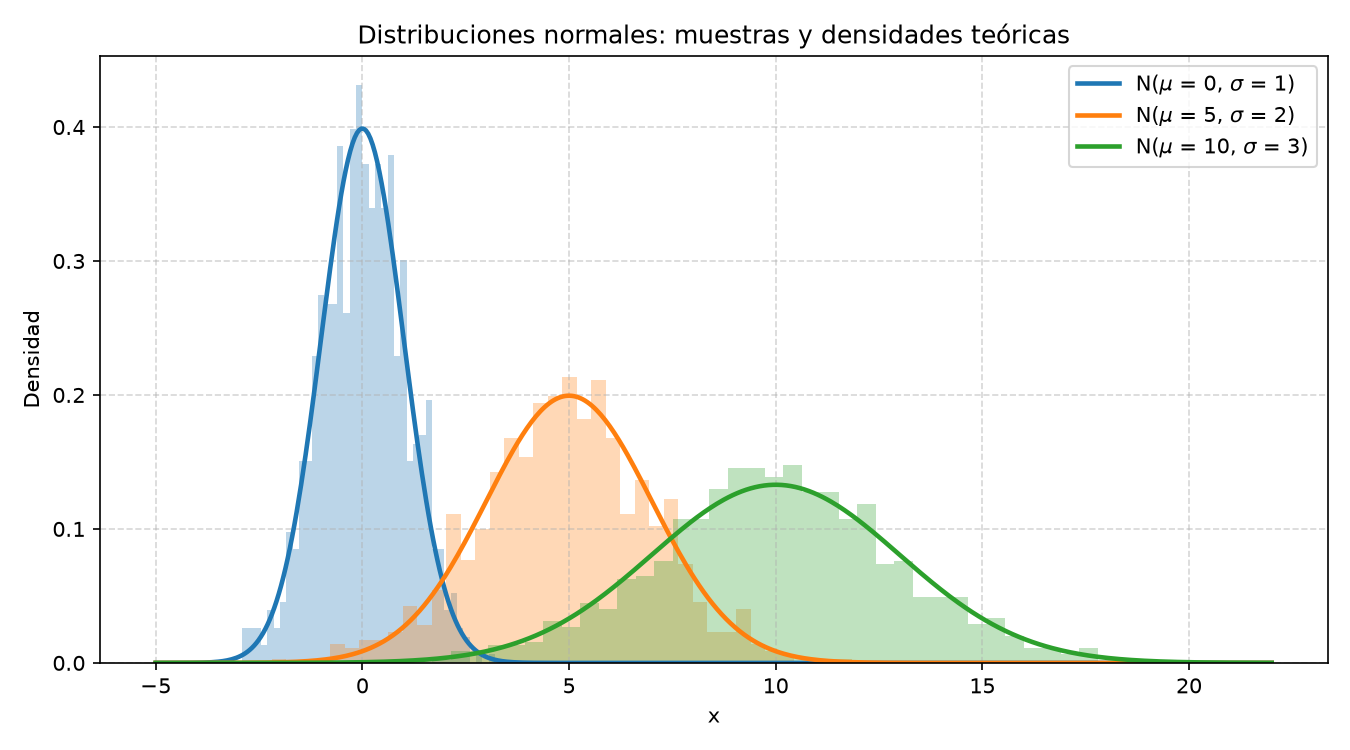
\includegraphics[width=0.85\textwidth]{img/a_normales.png}
\caption{Histogramas de 1000 muestras y densidades teóricas de $N(0, 1)$, $N(5, 2)$ y $N(10, 3)$.}
\label{fig:normales}
\end{figure}

\begin{figure}[htbp]
\centering
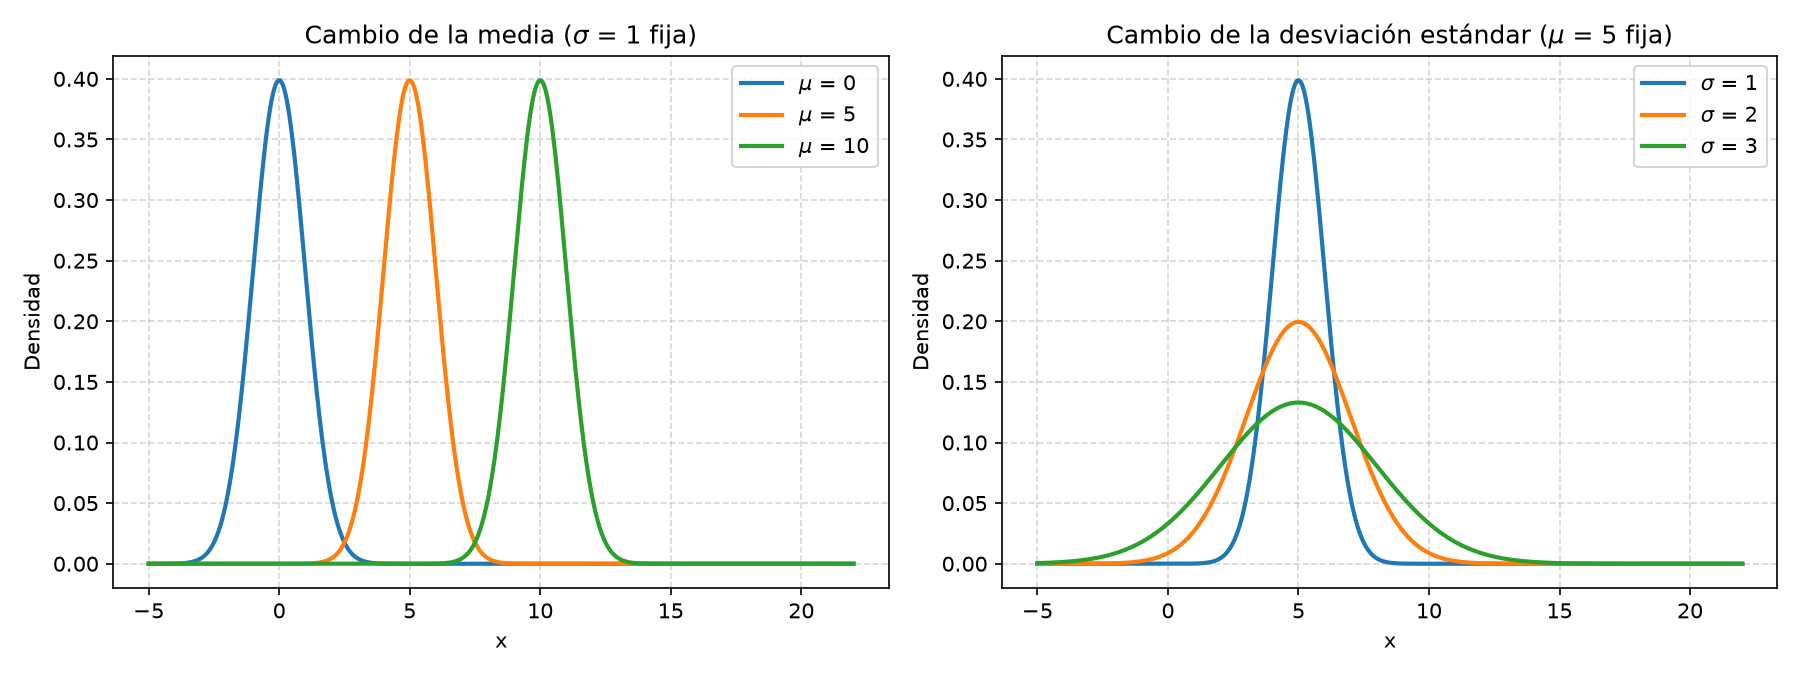
\includegraphics[width=\textwidth]{img/a_normales_parametros.png}
\caption{Efecto de cada parámetro por separado. Izquierda: cambio de la media con $\sigma = 1$. Derecha: cambio de la desviación estándar con $\mu = 5$.}
\label{fig:parametros}
\end{figure}

\begin{itemize}
    \item \textbf{Las muestras reproducen los parámetros.} Las medias muestrales (0.032, 4.916 y 9.985) y las desviaciones estándar (1.020, 2.062 y 2.892) quedan cerca de los valores poblacionales, y los histogramas de la Figura~\ref{fig:normales} siguen la forma de las curvas teóricas.
    \item \textbf{Efecto de la media.} En la Figura~\ref{fig:parametros} (izquierda), cambiar $\mu$ de 0 a 5 y a 10 desplaza la campana a la derecha sin modificar su forma: las tres curvas tienen la misma altura y el mismo ancho.
    \item \textbf{Efecto de la desviación estándar.} En la Figura~\ref{fig:parametros} (derecha), aumentar $\sigma$ de 1 a 3 ensancha la campana y baja su pico, de 0.399 a 0.199 y a 0.133. Es la relación $f(\mu) = 1/(\sigma\sqrt{2\pi})$: el área bajo la curva siempre es 1, por lo que una curva más ancha debe ser más baja.
    \item \textbf{Superposición.} En la Figura~\ref{fig:normales}, la curva con $\sigma = 1$ es alta y estrecha, concentrada entre $-2$ y 2, mientras que la de $\sigma = 3$ es baja y se extiende de 1 a 19 aproximadamente. Las curvas $N(5, 2)$ y $N(10, 3)$ se traslapan entre 4 y 10 aproximadamente, mientras que $N(0, 1)$ casi no se traslapa con las otras dos.
\end{itemize}

\subsection{Tarea b: Distribución de Poisson y comparación con la binomial}

\begin{consola}[label=out:b]{Ejecución de \texttt{act09.py}: Tarea b}
=== b) Distribución de Poisson: 1000 muestras por valor de lambda ===
 lambda  Media muestral  Varianza muestral  Moda  Máx. |empírica - teórica|
      1           0.987              0.976     1                      0.011
      5           4.972              4.696     4                      0.020
     10          10.035              9.589     9                      0.015

=== b) Comparación con binomiales de la misma media (n * p = lambda) ===
 lambda   n    p  Var. binomial  Var. Poisson  Dist. variación total
      1  20 0.05           0.95             1                 0.0142
      1 100 0.01           0.99             1                 0.0028
      5  20 0.25           3.75             5                 0.0714
      5 100 0.05           4.75             5                 0.0126
     10  20 0.50           5.00            10                 0.1665
     10 100 0.10           9.00            10                 0.0258
\end{consola}

\begin{figure}[htbp]
\centering
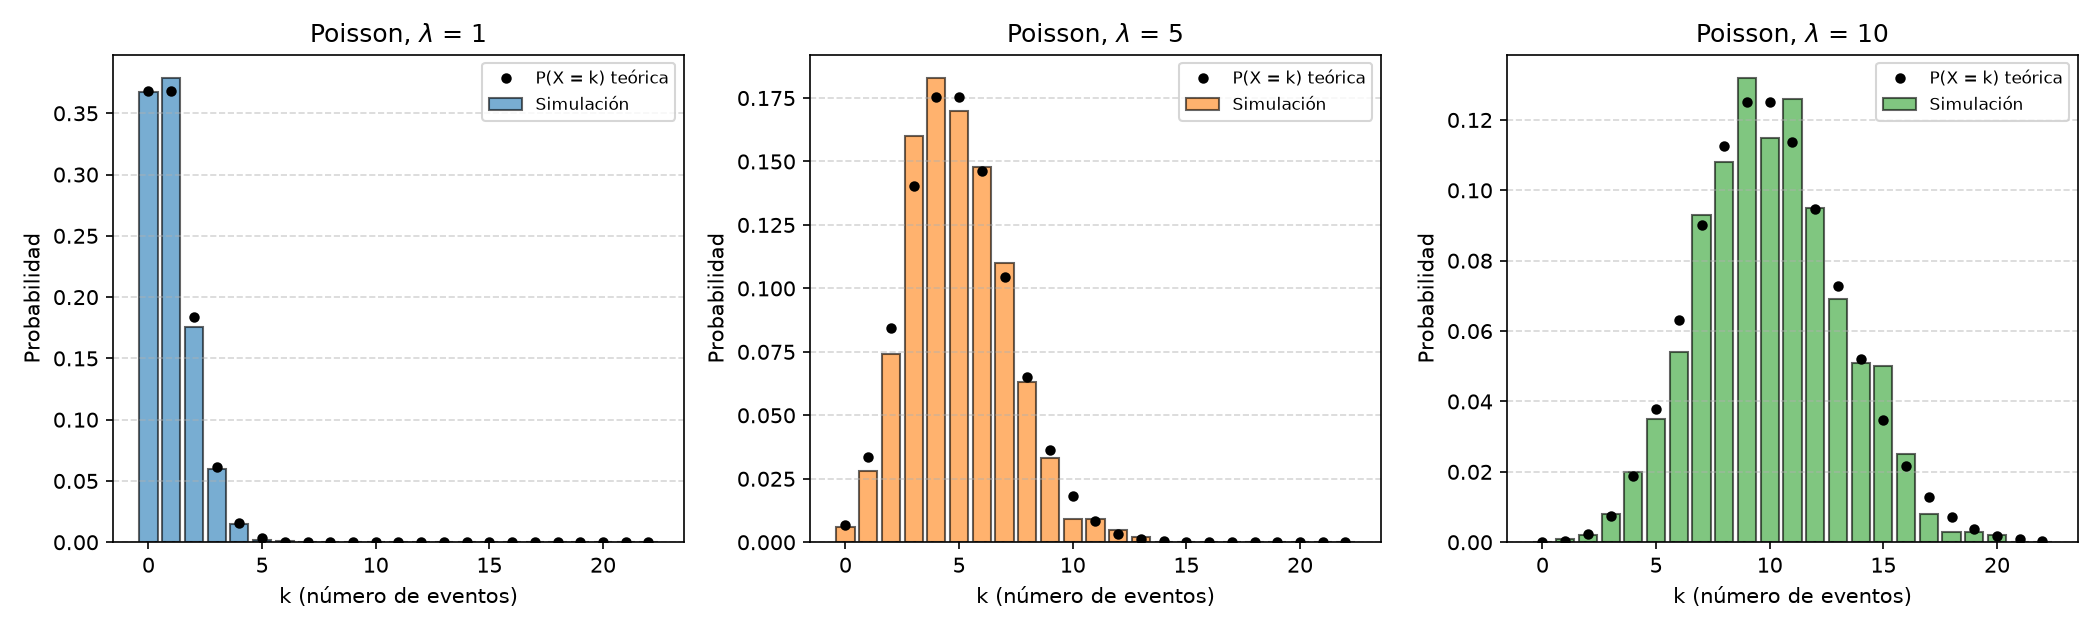
\includegraphics[width=\textwidth]{img/b_poisson.png}
\caption{Frecuencias relativas de 1000 valores simulados de una Poisson (barras) y función de masa teórica (puntos) para $\lambda = 1, 5$ y $10$.}
\label{fig:poisson}
\end{figure}

\begin{figure}[htbp]
\centering
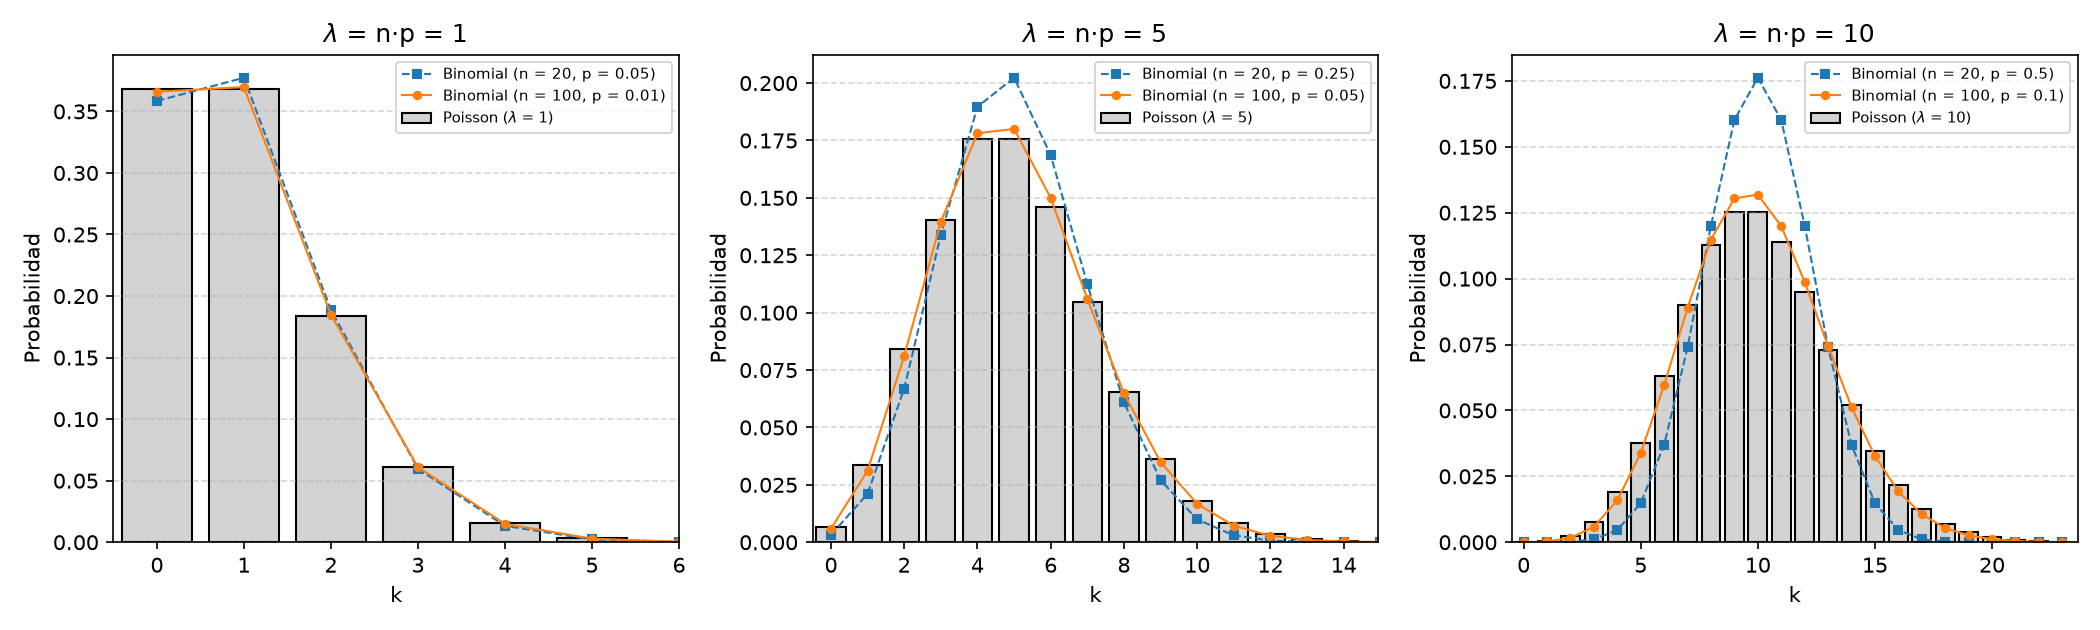
\includegraphics[width=\textwidth]{img/b_poisson_binomial.png}
\caption{Función de masa de Poisson (barras grises) y de binomiales con la misma media $np = \lambda$, con $n = 20$ y $n = 100$.}
\label{fig:poisson_binomial}
\end{figure}

\begin{itemize}
    \item \textbf{Forma según $\lambda$.} En la Figura~\ref{fig:poisson}, con $\lambda = 1$ la distribución es asimétrica: la probabilidad es máxima en 0 y en 1 (ambas $e^{-1} \approx 0.368$) y decrece rápidamente hacia la derecha. Con $\lambda = 5$ aparece un máximo en el centro y con $\lambda = 10$ la distribución es casi simétrica, con forma de campana, más baja y más ancha. Al aumentar $\lambda$ la distribución se desplaza a la derecha y se dispersa más.
    \item \textbf{Media igual a varianza.} Las medias muestrales (0.987, 4.972 y 10.035) y las varianzas muestrales (0.976, 4.696 y 9.589) son parecidas entre sí y a $\lambda$, como se espera de una Poisson, en la que ambas valen $\lambda$.
    \item \textbf{Moda.} Las modas observadas son 1, 4 y 9. Cuando $\lambda$ es un entero, la teoría da dos modas, $\lambda - 1$ y $\lambda$, con la misma probabilidad, por lo que en una muestra finita cualquiera de las dos puede ganar por azar.
    \item \textbf{Ajuste de la simulación.} La mayor diferencia entre la frecuencia observada y la teórica es de 0.011, 0.020 y 0.015 para los tres valores de $\lambda$, es decir, la simulación sigue la función de masa con diferencias de un par de puntos porcentuales o menos.
    \item \textbf{Comparación con la binomial.} En la Figura~\ref{fig:poisson_binomial}, la binomial con $n = 100$ casi coincide con la Poisson en los tres casos, y la distancia de variación total es 0.003, 0.013 y 0.026. Con $n = 20$ la diferencia es mayor y crece con $\lambda$ (0.014, 0.071 y 0.167), porque $p = \lambda/n$ ya no es pequeña: con $\lambda = 10$ y $p = 0.5$, la binomial tiene varianza $np(1-p) = 5$, la mitad que la Poisson (10), y por eso su campana es más alta y estrecha. Para $n = 100$ la varianza es 9, más cercana a 10. En todos los casos, la varianza binomial es menor que $\lambda$ por el factor $(1 - p)$, y la aproximación mejora cuando $n$ crece y $p$ disminuye, como indica la teoría \parencite{tecnm2026_documento_fuente}.
\end{itemize}

\subsection{Tarea c: Ajuste de una normal a la temperatura}

\begin{consola}[label=out:c]{Ejecución de \texttt{act09.py}: Tarea c}
=== c) Ajuste de una normal a la temperatura (Weather Dataset) ===
n = 14, mínimo = 64, máximo = 85
Media = 73.571, mediana = 72.0
Ajuste normal (máxima verosimilitud): mu = 73.571, sigma = 6.333
Desviación estándar muestral (n - 1): 6.572
Asimetría: 0.328   curtosis (exceso): -0.995
Prueba de Shapiro-Wilk: W = 0.9496, p = 0.5548

Frecuencias por intervalo:
Intervalo (°F)  Observadas  Esperadas (normal)
  [62.5, 67.5)           2                1.80
  [67.5, 72.5)           6                3.70
  [72.5, 77.5)           2                4.20
  [77.5, 82.5)           2                2.64
  [82.5, 87.5)           2                0.92

Figuras guardadas en img/
\end{consola}

\begin{figure}[htbp]
\centering
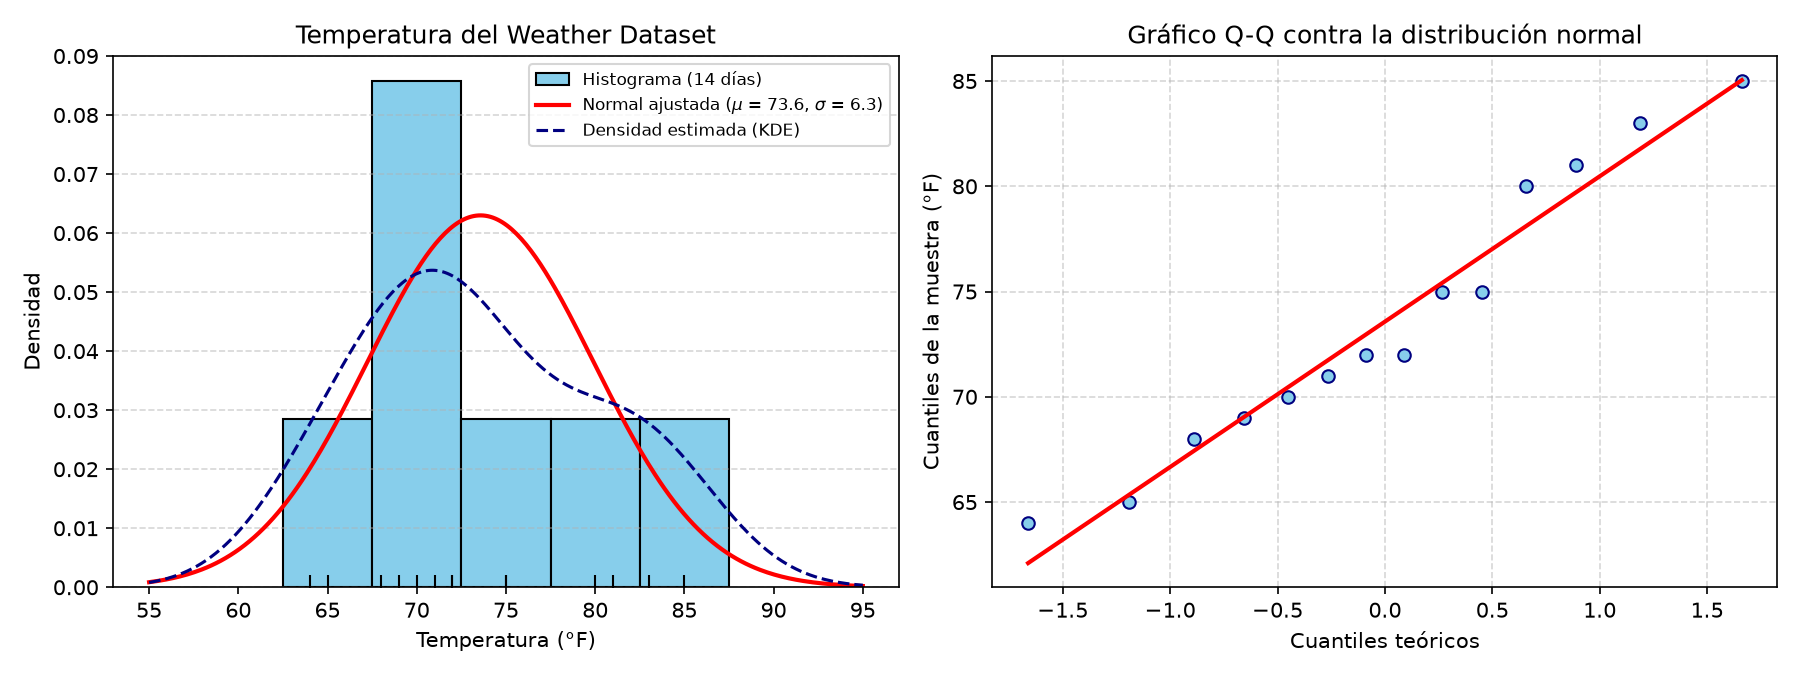
\includegraphics[width=\textwidth]{img/c_ajuste_temperatura.png}
\caption{Izquierda: histograma de la temperatura del Weather Dataset con la normal ajustada (rojo) y la densidad estimada por kernel (azul). Derecha: gráfico Q-Q contra la distribución normal.}
\label{fig:ajuste}
\end{figure}

\begin{itemize}
    \item \textbf{Parámetros ajustados.} La normal ajustada tiene $\mu = 73.57$\,°F y $\sigma = 6.33$\,°F (con divisor $n$; con $n - 1$ la desviación estándar es 6.57\,°F). La media y la mediana (72\,°F) son cercanas, y la asimetría es pequeña (0.33).
    \item \textbf{Histograma y curva.} En la Figura~\ref{fig:ajuste} (izquierda) el ajuste es solo aproximado. La normal captura el centro y el rango de los datos, pero el histograma no tiene forma de campana: tiene un intervalo alto en 67.5--72.5\,°F (6 de los 14 días, frente a 3.7 esperados) y los demás intervalos son planos con 2 días cada uno. La curtosis de $-0.995$ indica que los datos son más planos que una normal. La KDE, que no supone ninguna forma, se desplaza a la izquierda de la normal, con su máximo cerca de 71\,°F, y tiene una cola derecha más pesada.
    \item \textbf{Gráfico Q-Q.} En la Figura~\ref{fig:ajuste} (derecha) los puntos siguen razonablemente la recta, con desviaciones pequeñas en el centro y en la parte superior; no hay valores atípicos que se alejen de ella.
    \item \textbf{Prueba de normalidad.} La prueba de Shapiro-Wilk da $W = 0.9496$ y $p = 0.555$, por lo que no hay evidencia para rechazar la normalidad. Con solo 14 observaciones, la prueba tiene poco poder para detectar desviaciones, por lo que este resultado significa que los datos son compatibles con una normal, no que lo sean con certeza.
\end{itemize}

\section{Conclusiones}

La manipulación de los parámetros permitió ver el efecto de cada uno. En la normal, la media solo desplaza la curva y la desviación estándar controla su ancho y, por la restricción de que el área sea 1, también su altura: el pico baja de 0.399 a 0.133 cuando $\sigma$ pasa de 1 a 3. En la Poisson, el único parámetro $\lambda$ determina a la vez el centro y la dispersión (la media y la varianza son iguales), y la forma pasa de una distribución asimétrica con $\lambda = 1$ a una casi simétrica con $\lambda = 10$. Las simulaciones de 1000 valores reprodujeron las distribuciones teóricas con diferencias de unos pocos puntos porcentuales.

La comparación con la binomial confirmó que la Poisson es el límite de una binomial con $n$ grande y $p$ pequeño: con $n = 100$ la distancia de variación total fue de 0.026 como máximo, mientras que con $n = 20$ llegó a 0.167 cuando $p = 0.5$. Finalmente, el ajuste a la temperatura del Weather Dataset mostró que ajustar una distribución es un proceso en dos pasos, estimar los parámetros y evaluar el ajuste: con 14 observaciones, la normal con $\mu = 73.6$\,°F y $\sigma = 6.3$\,°F describe el centro y el rango, el gráfico Q-Q es razonablemente lineal y la prueba de Shapiro-Wilk no rechaza la normalidad, pero el histograma es más plano que una campana. Con una muestra tan pequeña no es posible distinguir con claridad entre una normal y otras formas, y la conclusión es que la normal es un modelo aceptable, no demostrado, para esta variable.

\referencias

\end{document}
